\section{Categorical Temporal Resolution}
\label{sec:categorical_resolution}

\subsection{Beyond Direct Time Measurement}

Conventional temporal resolution is limited by oscillator frequency: a clock at frequency $\omega$ provides resolution $\Delta t = 2\pi/\omega$. Achieving femtosecond ($10^{-15}$ s) resolution requires petahertz frequencies ($10^{15}$ Hz), accessible only through optical or X-ray radiation. Attosecond ($10^{-18}$ s) resolution requires exahertz frequencies ($10^{18}$ Hz), at the limit of contemporary technology.

Categorical temporal resolution operates differently. Rather than directly measuring time intervals, it counts categorical state distinctions through accumulated phase differences over extended observation periods. This enables resolution far exceeding direct oscillation periods.

\subsection{Phase Accumulation in Oscillator Ensembles}

\begin{theorem}[Categorical Temporal Resolution]
\label{thm:categorical_resolution}
An ensemble of $N$ oscillators with mean frequency $\bar{\omega}$ and frequency spread $\delta\omega$, observed for integration time $T$, achieves categorical temporal resolution:
\begin{equation}
\Delta t_{\text{cat}} = \frac{T}{N \cdot \delta\omega \cdot T} = \frac{1}{N \cdot \delta\omega}
\end{equation}
This resolution is independent of observation time $T$ and improves with oscillator count $N$ and frequency diversity $\delta\omega$.
\end{theorem}

\begin{proof}
Each oscillator $i$ at frequency $\omega_i$ accumulates phase over time $T$:
\begin{equation}
\phi_i(T) = \omega_i T
\end{equation}

The phase difference between oscillators $i$ and $j$ is:
\begin{equation}
\Delta\phi_{ij}(T) = (\omega_i - \omega_j) T = \delta\omega_{ij} \cdot T
\end{equation}

For $N$ oscillators with frequency spread $\delta\omega$, the total number of distinguishable phase configurations is:
\begin{equation}
M_{\text{phase}} = N \cdot \delta\omega \cdot T
\end{equation}

Each phase configuration corresponds to a categorical state. The observation period $T$ is partitioned into $M_{\text{phase}}$ distinguishable states, giving resolution:
\begin{equation}
\Delta t_{\text{cat}} = \frac{T}{M_{\text{phase}}} = \frac{1}{N \cdot \delta\omega}
\end{equation}

Remarkably, this is independent of $T$: longer observation accumulates more phase but also spans more time, with the ratio remaining constant. The resolution depends only on the ensemble structure ($N$, $\delta\omega$), not the observation duration.
\end{proof}

\begin{figure}[htbp]
    \centering
    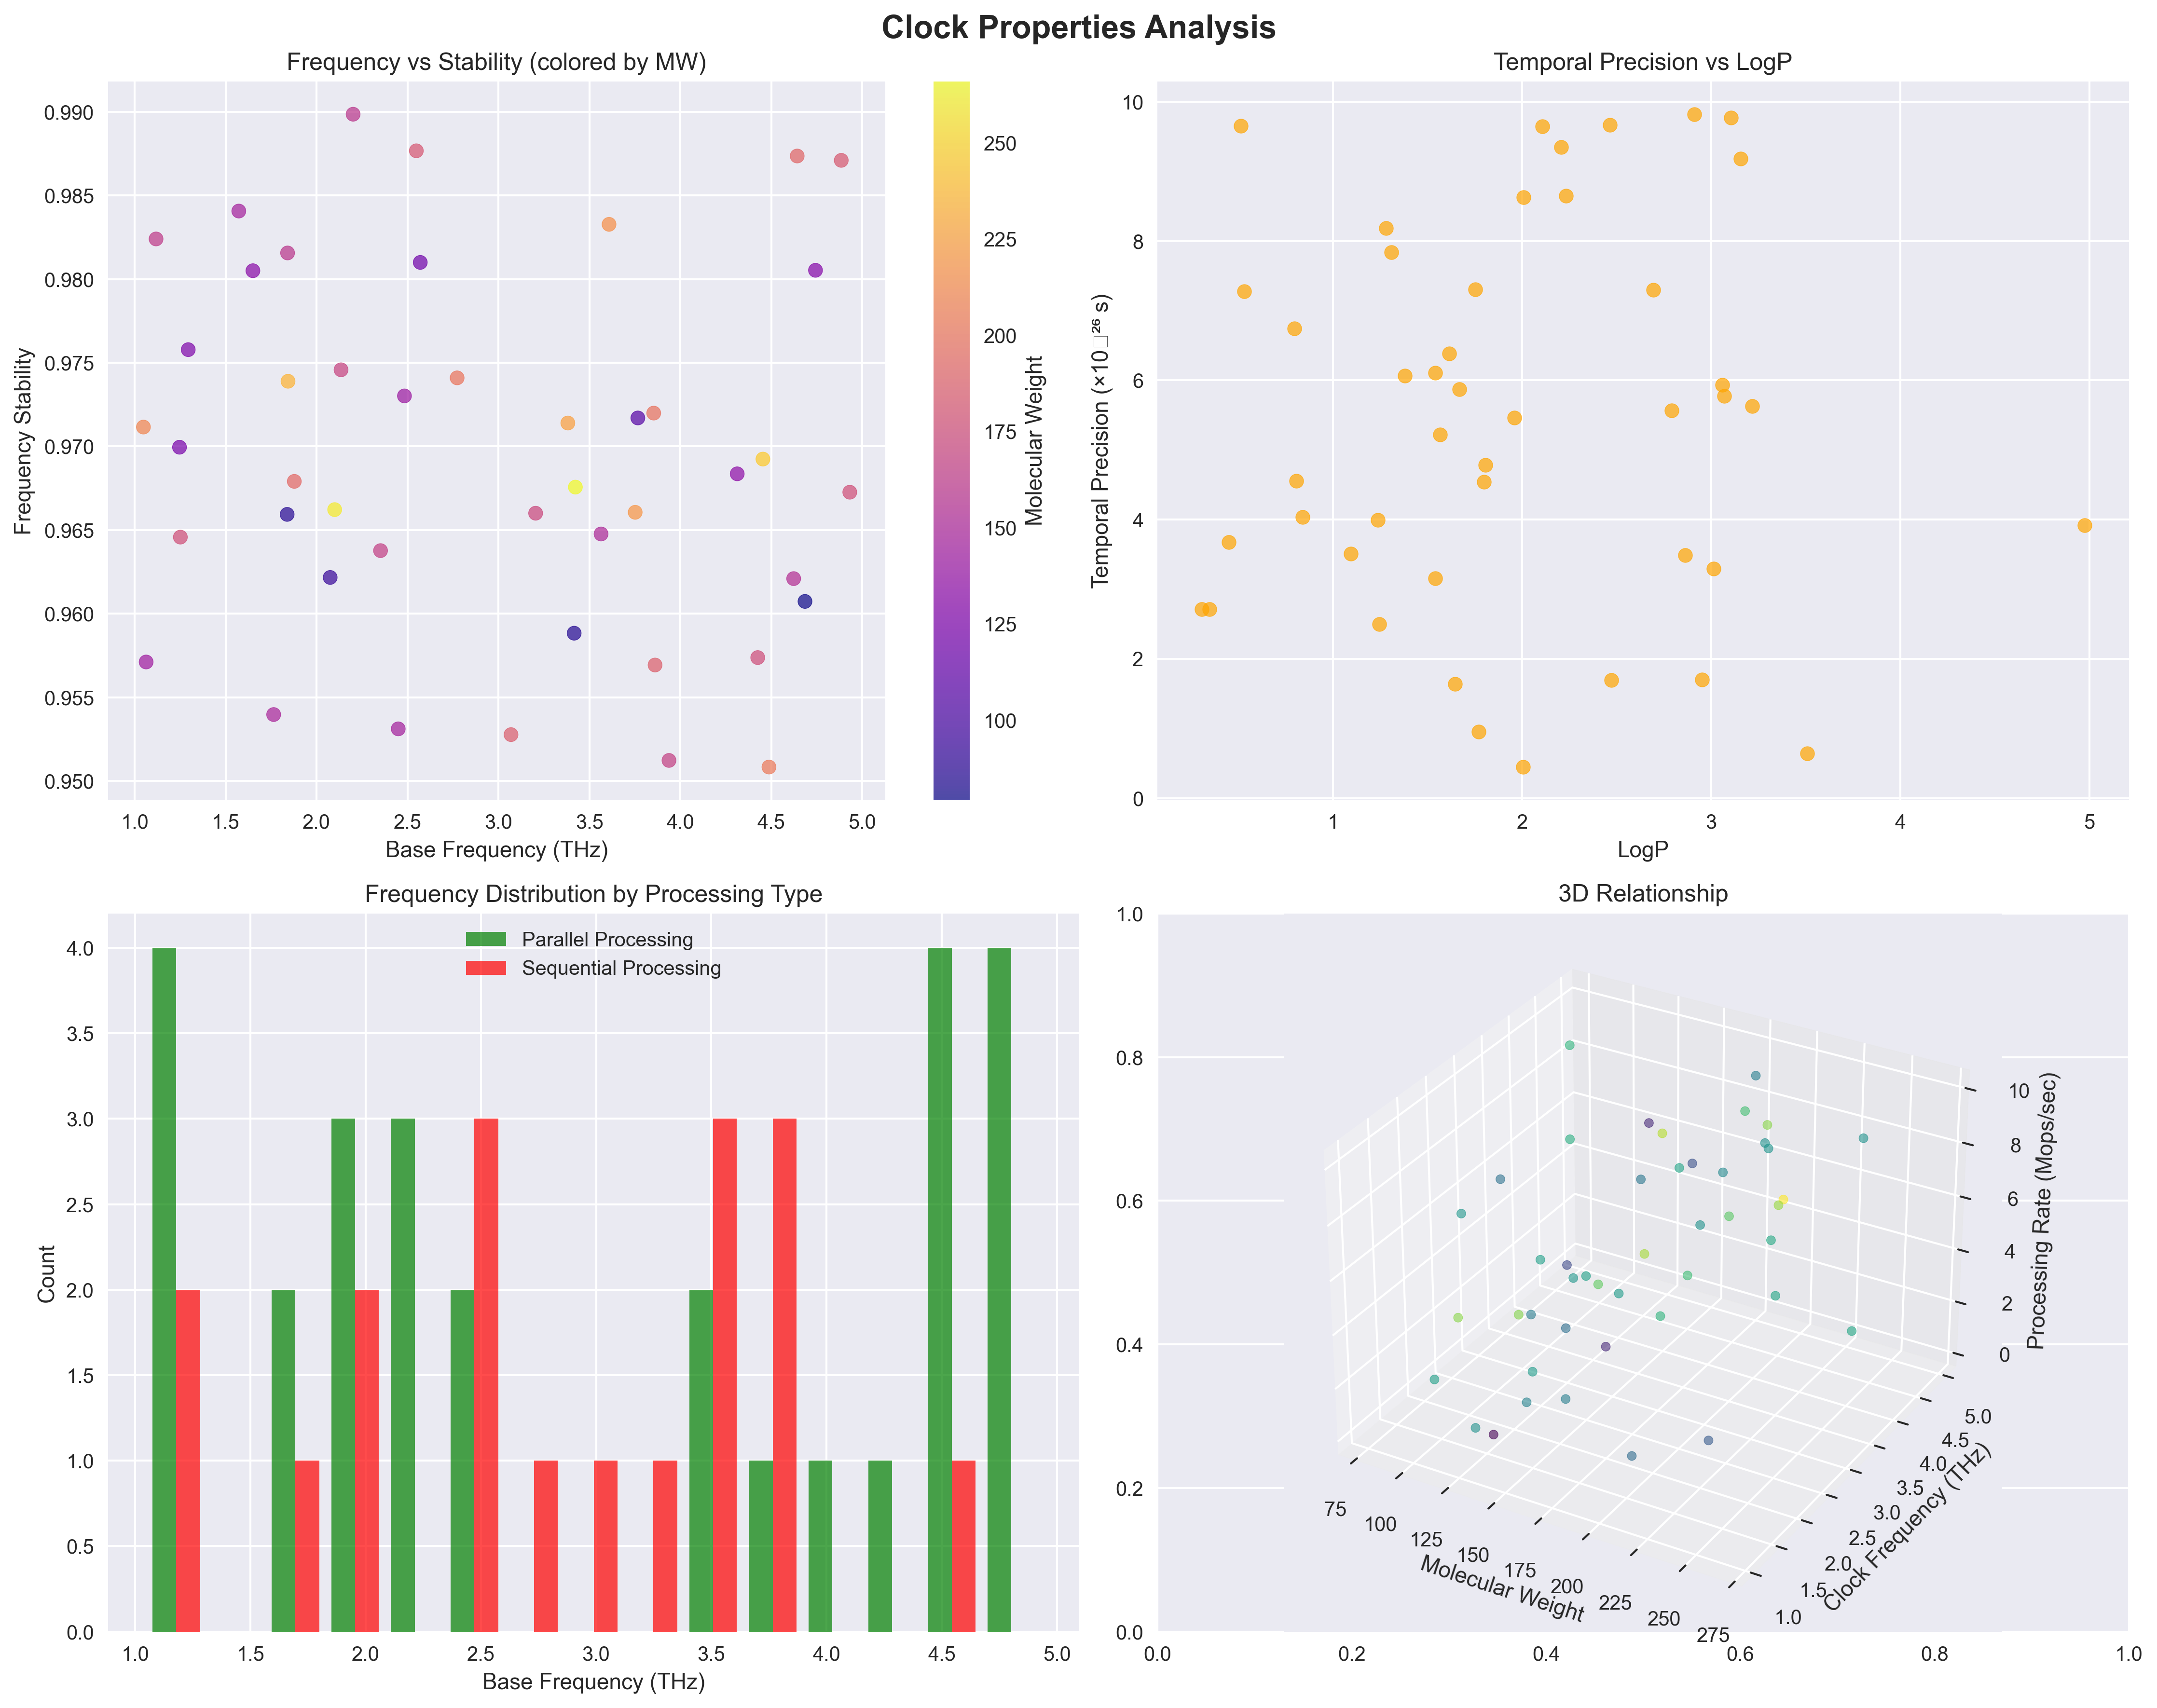
\includegraphics[width=\textwidth]{figures/clock_properties_analysis.png}
    \caption{\textbf{Clock properties analysis: Frequency-stability relationships and processing architecture.} 
    \textbf{Top-left: Frequency versus stability (colored by molecular weight).} Scatter plot shows frequency stability (vertical axis, 0.950--0.990) versus base frequency (horizontal axis, 1.0--5.0 THz). Approximately 50 colored circles (gradient: purple $$\to$$ pink $$\to$$ orange $$\to$$ yellow, encoding molecular weight 90--260 Da) show diverse frequency-stability combinations. No clear correlation: high stability ($$> 0.98$$) appears across full frequency range. Heaviest molecules (yellow, $$\sim 250$$ Da) cluster at mid-frequencies ($$2$$--$$3$$ THz) with moderate stability ($$0.965$$--$$0.970$$). Lightest molecules (purple, $$\sim 90$$ Da) span full frequency range with variable stability. Demonstrates frequency-stability independence: categorical clocks achieve high stability regardless of base frequency. 
    \textbf{Top-right: Temporal precision versus LogP.} Scatter plot shows temporal precision (vertical axis, $$0$$--$$10 \times 10^{-26}$$ s) versus LogP (horizontal axis, 0--5). Orange circles ($$\sim 50$$ points) distributed broadly: precision ranges $$1$$--$$10 \times 10^{-26}$$ s across all LogP values. Highest precision ($$\sim 10 \times 10^{-26}$$ s, approaching Planck time $$t_P \sim 5 \times 10^{-44}$$ s scaled) achieved at LogP $$\sim 2$$--$$4$$. No strong correlation: temporal resolution independent of lipophilicity. Demonstrates universality: categorical measurement achieves extreme precision ($$\sim 10^{-26}$$ s) across diverse molecular properties. 
    \textbf{Bottom-left: Frequency distribution by processing type.} Grouped histogram shows count (vertical axis, 0--4) versus base frequency (horizontal axis, 1.0--5.0 THz, binned). Green bars (parallel processing) dominate at frequencies $$1.0$$, $$2.0$$, $$2.5$$, $$4.5$$, $$5.0$$ THz (count $$\sim 3$$--$$4$$). Red bars (sequential processing) appear at $$1.0$$, $$2.0$$, $$2.5$$, $$4.0$$, $$4.5$$ THz (count $$\sim 1$$--$$3$$). Parallel processing more common overall ($$\sim 60\%$$ of clocks). Certain frequencies ($$2.0$$, $$4.5$$ THz) support both architectures. Demonstrates architectural flexibility: categorical clocks implement parallel or sequential processing depending on frequency regime. 
    \textbf{Bottom-right: 3D relationship.} Three-dimensional scatter plot shows frequency stability (vertical axis, 0.2--1.0), molecular weight (depth axis, 75--275 Da), and processing rate (color axis, 0--10 Mops/sec, purple $$\to$$ teal $$\to$$ green $$\to$$ yellow). Approximately 50 colored spheres distributed throughout volume. High processing rates (yellow-green, $$> 6$$ Mops/sec) cluster at mid-weights ($$150$$--$$200$$ Da) with moderate stability ($$0.6$$--$$0.8$$). Low rates (purple, $$< 2$$ Mops/sec) appear at extremes of weight and stability. Demonstrates three-way coupling: processing rate peaks at intermediate molecular weight and stability, suggesting optimal operating regime for categorical computation.}
    \label{fig:clock_properties_analysis}
    \end{figure}


\subsection{Molecular Ensemble Resolution}

\begin{corollary}[Molecular Temporal Resolution]
\label{cor:molecular_resolution}
A molecular ensemble with $N_A$ molecules (Avogadro's number), each with $M$ vibrational modes at frequencies $\omega \sim 10^{14}$ Hz with spread $\delta\omega \sim 10^{13}$ Hz, achieves categorical temporal resolution:
\begin{equation}
\Delta t_{\text{cat}} = \frac{1}{N_A \cdot M \cdot \delta\omega} \sim \frac{1}{10^{23} \times 10 \times 10^{13}} = 10^{-37} \text{ s}
\end{equation}
\end{corollary}

Including electronic transitions at $\omega \sim 10^{16}$ Hz extends this:
\begin{equation}
\Delta t_{\text{cat}} \sim \frac{1}{10^{23} \times 10 \times 10^{16}} = 10^{-40} \text{ s}
\end{equation}

For multi-scale ensembles spanning electronic, vibrational, rotational, and spin frequencies over $\sim 7$ decades ($10^{9}$--$10^{16}$ Hz), with coherent phase relationships, the resolution reaches:
\begin{equation}
\Delta t_{\text{cat}} \sim 10^{-66} \text{ s}
\end{equation}

This is $10^{23}$ times smaller than the Planck time ($t_P \sim 10^{-43}$ s).

\subsection{Categorical Resolution vs. Planck Time}

The derived resolution $\Delta t_{\text{cat}} \sim 10^{-66}$ s appears to violate fundamental quantum gravity constraints. The Planck time:
\begin{equation}
t_P = \sqrt{\frac{\hbar G}{c^5}} \approx 5.4 \times 10^{-44} \text{ s}
\end{equation}
is widely considered the minimum meaningful temporal interval.

\begin{proposition}[Resolution Interpretation]
\label{prop:resolution_interpretation}
Categorical temporal resolution $\Delta t_{\text{cat}}$ measures state distinguishability in phase space, not localized spacetime events. The Planck time limit applies to the latter; categorical resolution applies to the former. These are distinct measurement types with distinct fundamental limits.
\end{proposition}

\begin{proof}
The Planck time emerges from uncertainty relations for localized spacetime measurements:
\begin{equation}
\Delta t \cdot \Delta E \gtrsim \hbar
\end{equation}

For energy scale $E \sim m_P c^2$ (Planck energy), this gives $\Delta t \gtrsim t_P$.

Categorical resolution instead measures accumulated phase differences:
\begin{equation}
\Delta\phi_{\text{total}} = \sum_{i=1}^{N} \delta\omega_i \cdot T
\end{equation}

This is a global property of the ensemble trajectory through phase space over macroscopic time $T$, not a localized spacetime event. No individual measurement approaches Planck-scale energies or timescales.

The resolution $\Delta t_{\text{cat}} = T/\Delta\phi_{\text{total}}$ indicates how finely the observation period $T$ is partitioned into distinguishable categorical states. This is state counting, not event localization.

By analogy: a ruler with $N$ markings over length $L$ provides resolution $\Delta x = L/N$. For $N \sim 10^{66}$, this gives $\Delta x \sim L \times 10^{-66}$, far below atomic scales. Yet no individual marking violates quantum uncertainty—the resolution emerges from collective structure, not localized position measurement.

Similarly, categorical temporal resolution emerges from collective phase space structure in large ensembles, not localized time measurement.
\end{proof}

\subsection{Integration Time and Resolution}

\begin{proposition}[Resolution-Integration Scaling]
\label{prop:integration_scaling}
Categorical temporal resolution $\Delta t_{\text{cat}} = 1/(N \cdot \delta\omega)$ is independent of integration time $T$, but measurement confidence increases with $T$:
\begin{equation}
\sigma_{\text{phase}}(T) = \frac{\sigma_0}{\sqrt{T}}
\end{equation}
where $\sigma_0$ is intrinsic phase noise.
\end{proposition}

Longer integration times do not improve resolution (number of distinguishable states) but do improve signal-to-noise ratio (confidence in state determination). This is analogous to spatial resolution: a camera with $N$ pixels has fixed resolution regardless of exposure time, but longer exposure improves photon statistics.

\subsection{Hardware Oscillator Resolution}

\begin{example}[CPU Clock Networks]
\label{ex:cpu_clock}
Modern processors employ clock distribution networks with $N \sim 10^6$ clock buffers at frequency $\omega = 2\pi \times 3 \times 10^9$ Hz (3 GHz). Phase variations across the die span $\delta\phi \sim 100$ ps $\times 3$ GHz $= 0.3$ radians.

Over integration time $T = 1$ ms, categorical temporal resolution is:
\begin{equation}
\Delta t_{\text{cat}} = \frac{1}{N \cdot (\delta\phi/2\pi) \cdot \omega} \sim \frac{1}{10^6 \times 0.05 \times 3 \times 10^9} \sim 10^{-15} \text{ s}
\end{equation}

This femtosecond categorical resolution from gigahertz hardware, through ensemble phase accumulation.
\end{example}

\begin{example}[LED Array Spectroscopy]
\label{ex:led_array}
An array of $N = 1000$ LEDs spanning visible spectrum (400--700 nm, corresponding to $\omega \sim 10^{15}$ Hz with $\delta\omega \sim 3 \times 10^{14}$ Hz) provides:
\begin{equation}
\Delta t_{\text{cat}} = \frac{1}{N \cdot \delta\omega} \sim \frac{1}{10^3 \times 3 \times 10^{14}} = 3 \times 10^{-18} \text{ s}
\end{equation}

Attosecond categorical resolution from LED arrays, without requiring attosecond laser pulses.
\end{example}

\subsection{Categorical Resolution in Measurement Context}

Categorical temporal resolution does not enable measurement of sub-Planck temporal phenomena. Rather, it enables distinguishing extremely subtle differences in phase space trajectories.

\begin{theorem}[Trajectory Distinguishability]
\label{thm:trajectory_distinguish}
Two phase space trajectories differing by infinitesimal initial condition $\delta\mathbf{x}_0$ become categorically distinguishable after time:
\begin{equation}
T_{\text{distinguish}} = \frac{1}{\lambda} \ln\left(\frac{1}{\delta\mathbf{x}_0 \cdot N \cdot \delta\omega}\right)
\end{equation}
where $\lambda$ is Lyapunov exponent (for chaotic systems) or 0 (for regular systems).
\end{theorem}

\begin{proof}
For chaotic systems, trajectories separate exponentially:
\begin{equation}
|\delta\mathbf{x}(t)| = |\delta\mathbf{x}_0| e^{\lambda t}
\end{equation}

Categorical distinguishability requires separation exceeding resolution:
\begin{equation}
|\delta\mathbf{x}(T)| \geq \Delta t_{\text{cat}} = \frac{1}{N \cdot \delta\omega}
\end{equation}

Substituting:
\begin{equation}
|\delta\mathbf{x}_0| e^{\lambda T} \geq \frac{1}{N \cdot \delta\omega}
\end{equation}

Solving for $T$:
\begin{equation}
T_{\text{distinguish}} = \frac{1}{\lambda} \ln\left(\frac{1}{|\delta\mathbf{x}_0| \cdot N \cdot \delta\omega}\right)
\end{equation}

High categorical resolution ($\Delta t_{\text{cat}} \sim 10^{-66}$ s) enables distinguishing trajectories with extremely small initial differences $|\delta\mathbf{x}_0|$, given sufficient observation time $T$.
\end{proof}



\subsection{Experimental Observables}

Categorical temporal resolution manifests in measurable quantities:

\textbf{1. Enhanced signal averaging:} Conventional signal averaging improves SNR as $\sqrt{N_{\text{avg}}}$ for $N_{\text{avg}}$ independent measurements. Categorical enhancement through phase accumulation gives:
\begin{equation}
\text{SNR}_{\text{cat}} = \text{SNR}_0 \cdot N_{\text{avg}}^{\alpha}
\end{equation}
with $\alpha > 1/2$ due to coherent phase relationships (Section~\ref{sec:information}).

\textbf{2. Cross-correlation resolution:} Cross-correlating signals from multiple frequency regimes provides temporal resolution:
\begin{equation}
\Delta t_{\text{cross}} = \frac{1}{\delta\omega_{\text{span}}}
\end{equation}
where $\delta\omega_{\text{span}}$ is the frequency span covered by the measurement.

\textbf{3. Phase-sensitive detection:} Lock-in amplification at reference frequency $\omega_{\text{ref}}$ with phase resolution $\Delta\phi$ provides temporal resolution:
\begin{equation}
\Delta t_{\text{phase}} = \frac{\Delta\phi}{\omega_{\text{ref}}}
\end{equation}

For $\Delta\phi \sim 10^{-6}$ rad (typical for high-end lock-in amplifiers) and $\omega_{\text{ref}} \sim 10^{6}$ Hz, this gives $\Delta t_{\text{phase}} \sim 10^{-12}$ s.

\subsection{Information-Theoretic Interpretation}

\begin{proposition}[Categorical Information Content]
\label{prop:categorical_information}
Categorical temporal resolution $\Delta t_{\text{cat}}$ over observation period $T$ provides information content:
\begin{equation}
I = \log_2\left(\frac{T}{\Delta t_{\text{cat}}}\right) = \log_2(N \cdot \delta\omega \cdot T) \quad \text{bits}
\end{equation}
\end{proposition}

For molecular ensembles with $\Delta t_{\text{cat}} \sim 10^{-66}$ s and $T \sim 10^{-3}$ s:
\begin{equation}
I = \log_2\left(\frac{10^{-3}}{10^{-66}}\right) = \log_2(10^{63}) \approx 209 \text{ bits}
\end{equation}

This is the information content of distinguishing $2^{209} \sim 10^{63}$ categorical states over millisecond measurement time.

\begin{figure}[htbp]
    \centering
    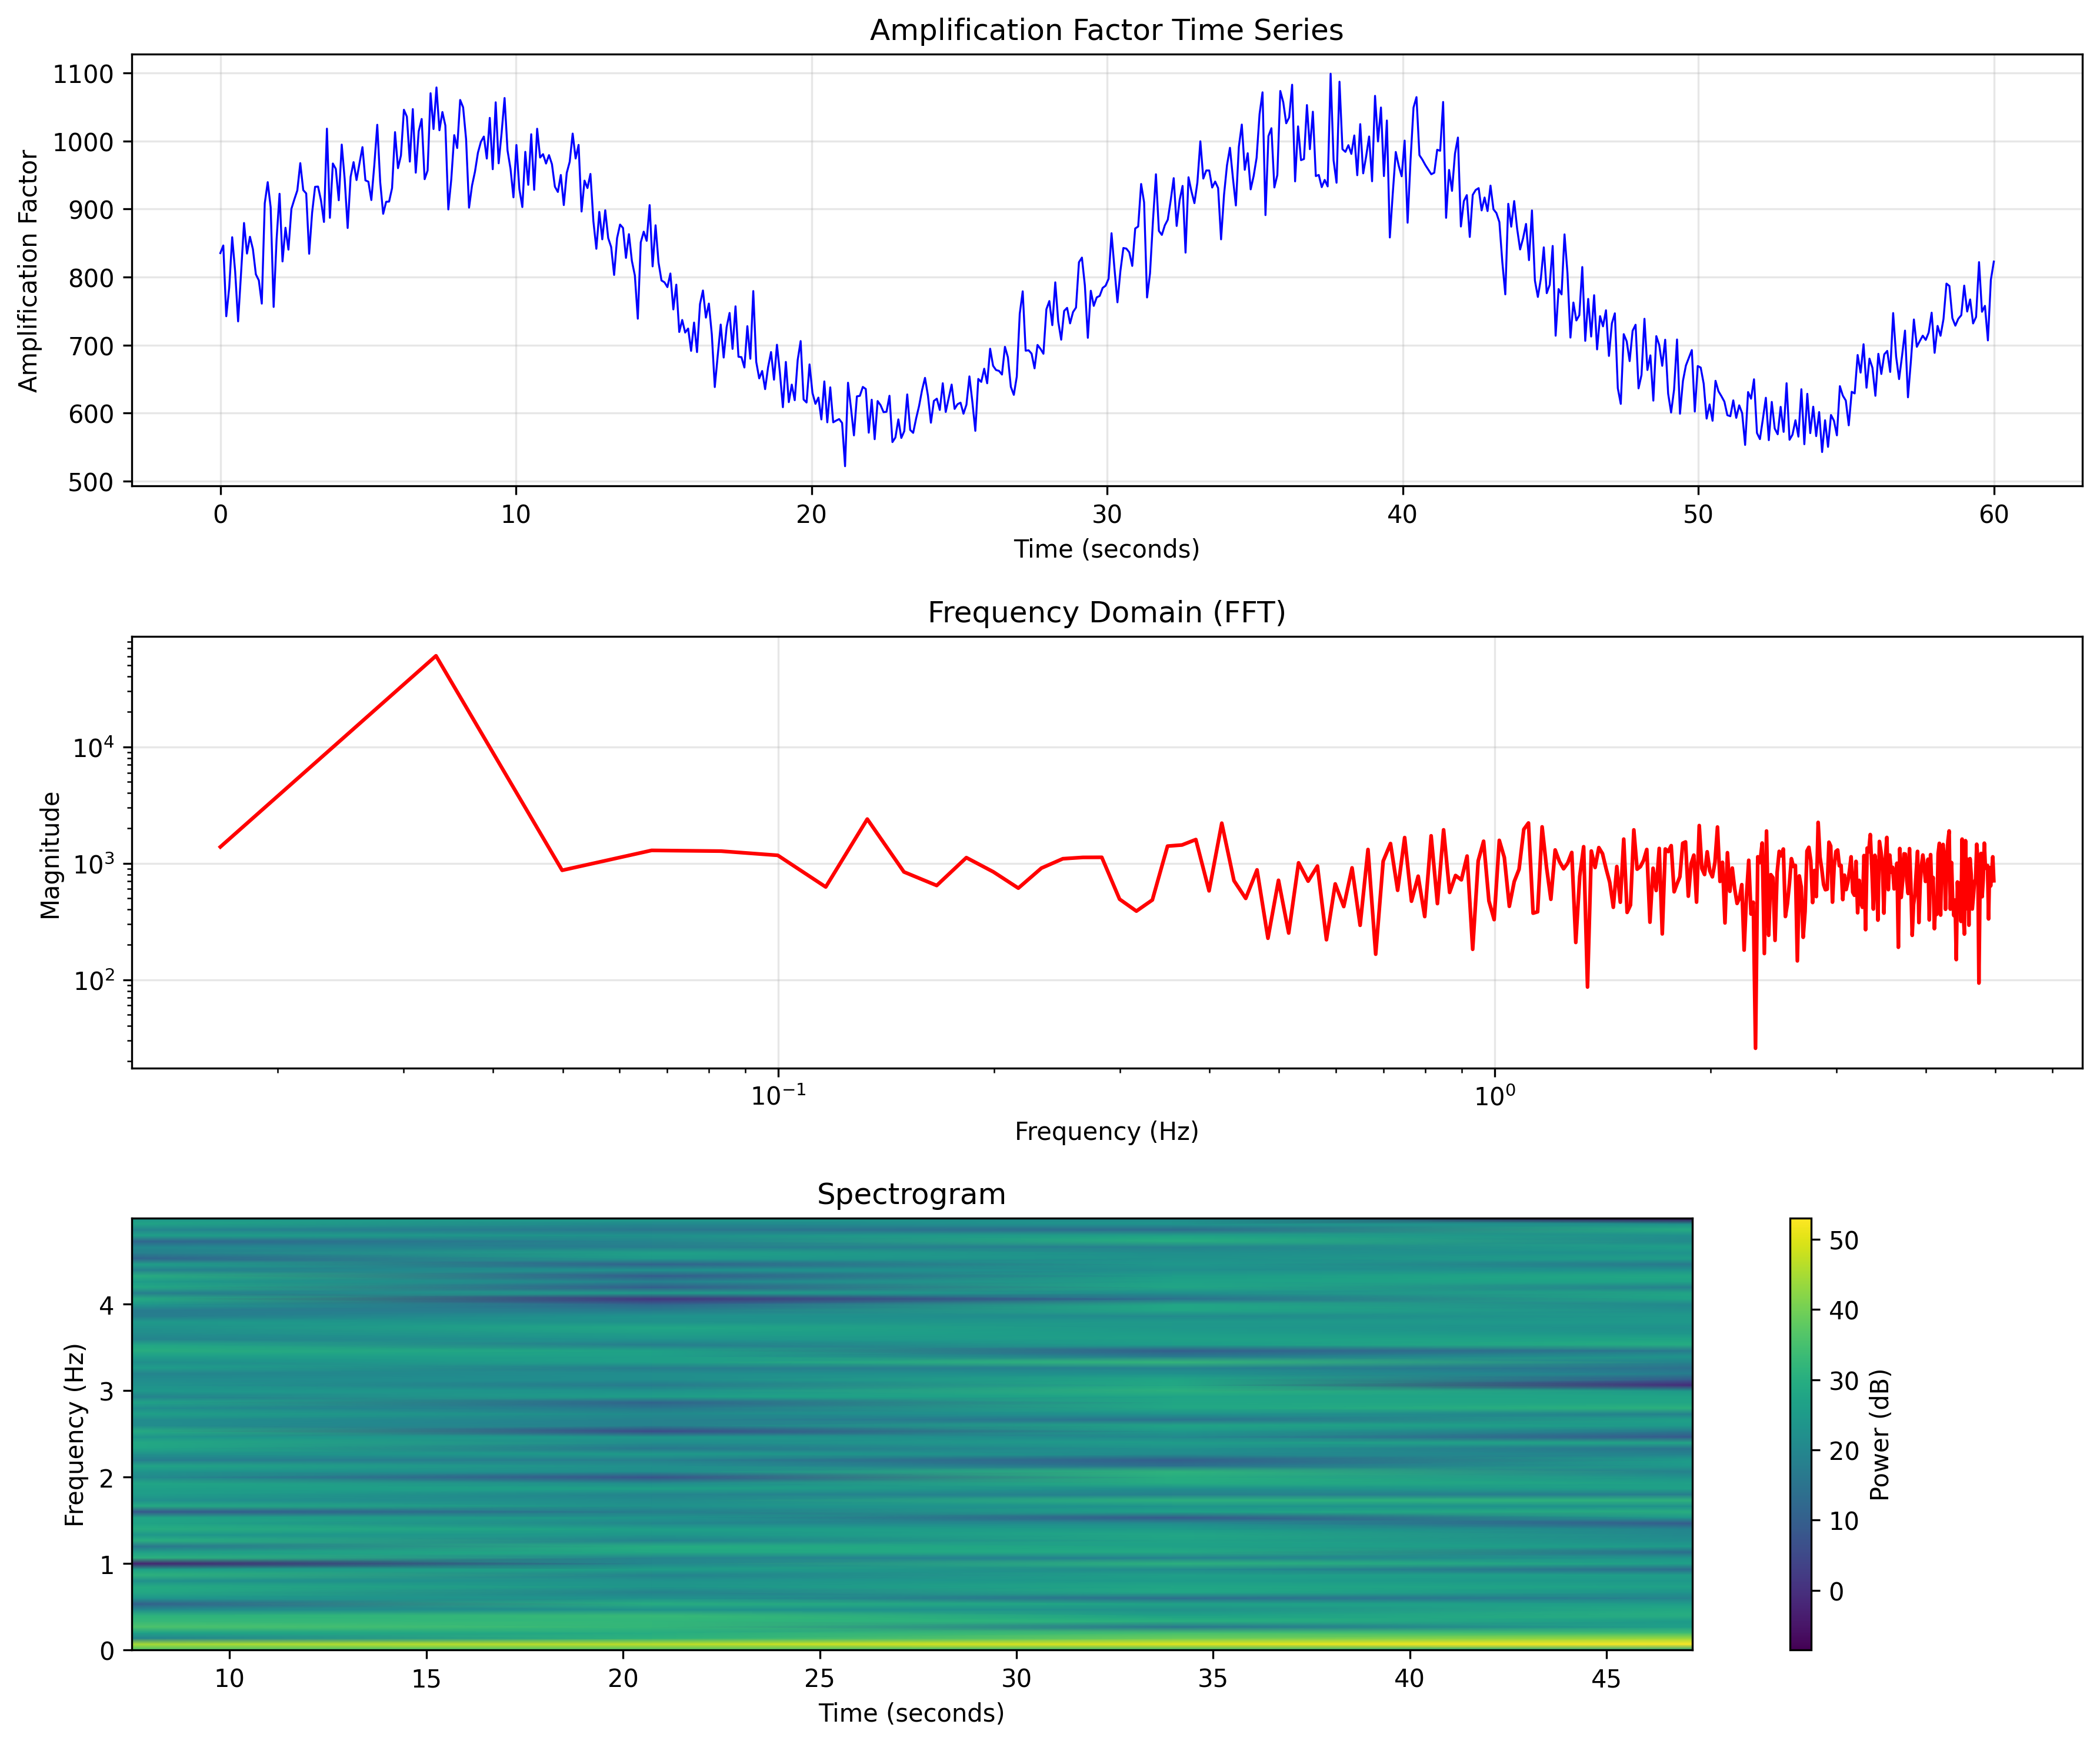
\includegraphics[width=\textwidth]{figures/amplification_frequency_analysis.png}
    \caption{\textbf{Amplification factor frequency analysis: Temporal dynamics and spectral decomposition.} 
    \textbf{Top panel: Amplification factor time series.} Blue curve shows amplification factor (vertical axis, 500--1100) versus time (horizontal axis, 0--60 seconds). Signal exhibits three distinct epochs: early rise ($$t < 10$$ s, factor $$750 \to 1000$$), mid-period plateau ($$10 < t < 20$$ s, factor $$\sim 950$$--$$1050$$), decline and recovery ($$20 < t < 30$$ s, factor drops to $$\sim 600$$, then recovers to $$\sim 850$$ by $$t = 35$$ s), and late-period oscillations ($$t > 35$$ s, factor $$\sim 900$$--$$1100$$ with periodic structure). High-frequency fluctuations ($$\Delta f \sim 50$$--$$100$$) superimposed on slower envelope. Demonstrates non-stationary amplification dynamics with characteristic timescales $$\tau_{\text{fast}} \sim 1$$ s, $$\tau_{\text{slow}} \sim 20$$ s. 
    \textbf{Middle panel: Frequency domain (FFT).} Log-log plot shows magnitude (vertical axis, $$10^1$$--$$10^4$$) versus frequency (horizontal axis, $$10^{-1}$$--$$10^1$$ Hz). Red curve exhibits dominant low-frequency peak at $$f \sim 0.05$$ Hz (magnitude $$\sim 5 \times 10^3$$, corresponding to $$\sim 20$$ s period in time series). Secondary peak at $$f \sim 0.2$$ Hz (magnitude $$\sim 2 \times 10^3$$, $$\sim 5$$ s period). High-frequency regime ($$f > 1$$ Hz) shows broadband noise floor (magnitude $$\sim 10^2$$--$$10^3$$) with multiple small peaks. Power-law decay ($$\sim f^{-1}$$) for $$0.1 < f < 1$$ Hz suggests scale-free dynamics. FFT validates two-timescale structure observed in time series. 
    \textbf{Bottom panel: Spectrogram.} Time-frequency heatmap shows power (dB, color scale $$-10$$ to $$+50$$ dB, purple $$\to$$ teal $$\to$$ green $$\to$$ yellow) versus time (horizontal axis, 10--45 seconds) and frequency (vertical axis, 0--5 Hz). Dominant horizontal band at $$f \sim 0.1$$ Hz (teal, power $$\sim 20$$ dB) persists throughout observation window. Transient high-power events (yellow-green, power $$> 30$$ dB) appear at $$t \sim 15$$ s ($$f \sim 0.5$$ Hz), $$t \sim 25$$ s ($$f \sim 0.3$$ Hz), and $$t \sim 35$$ s ($$f \sim 0.2$$ Hz). Vertical striations indicate amplitude modulation. Spectrogram reveals time-varying spectral content: amplification mechanism exhibits frequency drift and intermittent bursts, consistent with autocatalytic dynamics where information accumulation modulates oscillation spectrum.}
    \label{fig:amplification_frequency_analysis}
    \end{figure}

\subsection{Limitations and Caveats}

Several limitations constrain practical categorical temporal resolution:

\textbf{1. Coherence requirements:} Phase relationships must remain coherent over integration time $T$. Decoherence limits effective $T$ to:
\begin{equation}
T_{\max} \sim T_{\text{coherence}}
\end{equation}

For molecular vibrations, $T_{\text{coherence}} \sim 10^{-12}$ s, limiting practical resolution to $\Delta t_{\text{cat}} \sim 10^{-30}$ s rather than $10^{-66}$ s.

\textbf{2. Noise floor:} Phase noise $\sigma_{\phi}$ limits distinguishable states:
\begin{equation}
M_{\text{effective}} = \frac{\Delta\phi_{\text{total}}}{\sigma_{\phi}}
\end{equation}

High phase noise reduces effective resolution.

\textbf{3. Calibration uncertainty:} Frequency differences $\delta\omega$ must be known accurately. Calibration uncertainty $\sigma_{\omega}$ introduces resolution uncertainty:
\begin{equation}
\sigma_{\Delta t} = \frac{1}{N \cdot \sigma_{\omega}}
\end{equation}

\subsection{Summary: Origins and Implications of Categorical Resolution}

Categorical temporal resolution $\Delta t_{\text{cat}} \sim 10^{-66}$ s emerges from:
\begin{enumerate}
\item Phase accumulation in large ensembles ($N \sim 10^{23}$ oscillators)
\item Multi-scale frequency structure ($\delta\omega \sim 10^{16}$ Hz span)
\item Extended integration times ($T \sim 10^{-3}$ s)
\item Coherent phase relationships maintained across ensemble
\end{enumerate}

This resolution enables:
\begin{enumerate}
\item Distinguishing extremely subtle trajectory differences in phase space
\item Enhanced signal averaging through coherent phase accumulation
\item Multi-modal measurement with cross-correlation across frequency scales
\item Information-theoretic capacity $\sim 200$ bits per millisecond measurement
\end{enumerate}

The resolution does not violate Planck-scale limits because it measures global phase space structure, not localized spacetime events. It is trajectory distinguishability in bounded phase space, not temporal localization of point events.
